\section{Свободная группа. Теорема о том, что всякая группа есть факторгруппа свободной группы.}

Пусть $ S = \{ a, b, c \cdots \}, \; S^{-1} = \{ a^{-1}, b^{-1}, c^{-1}, \cdots \} $. 
Будем называть $ A = S \cup S^{-1} $ \emph{алфавитом}, а $ A^{*} $ - множеством всевозможных слов над алфавитом $ A $.
\emph{Пустым} словом будем называть $ aa^{-1} = \emptyset $. Введем отношение эквивалентности на $ A^{*} $. $ w \sim v $, если 
$ w $ можно получить из $ v $ с помощью правил сокращения. Также введем операцию \emph{конкатенации} на $ A^{*} $.

\begin{defn}
  $ F_{S} = A^{*} \cup \emptyset /\!\!\!\sim $ - группа по конкатенации. 
  $ F_{S} $ - \emph{свободная группа}, порожденная $ S $.
\end{defn}

\begin{thm}[Категорное свойство свободной группы]
  Существует единственный гомоморфизм, делающий диаграмму коммутативной. 
  То есть $ \forall f : S \rightarrow G \;\; \exists ! \phi_{f} : F_{S} \rightarrow G, \;\; f = \phi_{f} \circ i $. \newline
  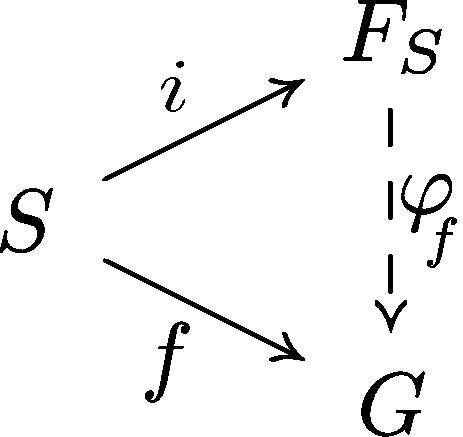
\includegraphics[scale=0.3]{question8_1}
\end{thm}
\begin{proof}
  Пусть $ S = \{ s_{1}, \cdots, s_{n} \} $. Тогда $ Im f = \{ f(s_{1}, \cdots, f(s_{n}) \} = \{ g_{1}, \cdots, g_{n} \} $. Теперь
  введем $ \phi_{f}(s_{1}^{n_{1}}s_{2}^{n_{2}}\cdots s_{i}^{n_{i}}) = g_{2}^{n_{1}}g_{2}^{n_{2}}\cdots g_{i}^{n_{i}} $. Единственность
  очевидна по построению.
\end{proof}

\begin{thm}
  Приведенное выше свойство может быть принято за определение свободной группы с точностью до изоморфизма.
\end{thm}
\begin{proof}
  Пусть существуют две свободные группы, порожденные $ S $ : $ F_{1} $ и $ F_{2} $. Тогда по свойству
  существуют единственные гомоморфизмы $ \phi_{i} : F_{1} \rightarrow F_{2} $ и $ \phi_{j} : F_{2} \rightarrow F_{1} $. А это значит, что
  $ F_{1} \overset\sim{=} F_{2} $. \newline
  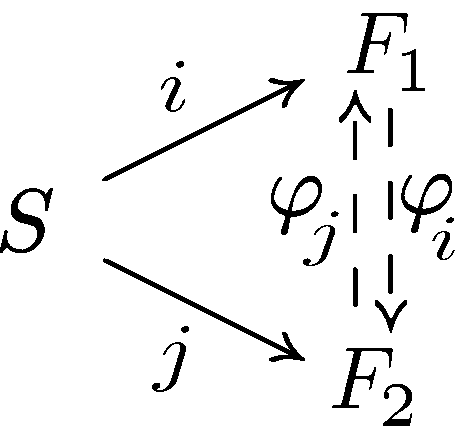
\includegraphics[scale = 0.3]{question8_2.pdf}
\end{proof}

\pagebreak

\begin{thm}
  Любая группа есть факторгруппа некоторой свободной группы.
\end{thm}
\begin{proof}
  Пусть $ G $ - группа. Забудем о её груповых свойствах и рассмотрим как множество. 
  Рассмотрим $ F_{G} $ - свободную группу, порожденную $ G $. Теперь вспомним
  о том, что $ G $ - группа. Тогда $ \exists \phi : F_{G} \rightarrow G $ - 
  естественный эпиморфизм групп, то есть $ Im \, \phi = G $. По основной теореме о гомоморфизме 
  $ F_{G}/ker \phi \overset\sim{=} Im \, \phi = G $. 
\end{proof}

Пример:

$ F_{ \{a,b\} } \overset\sim{=} \mathbb{Z} \times \mathbb{Z} $, если введены следующие правила $ aba^{-1}b^{-1} = e, ab = ba $.
